Die Minimalstandards des Veranstaltungsangebots stellen Forderungen an die Konzeption der mathematischen und mathematikverwandten Studiengänge.

In allen ist eine gewisse fachliche Breite und die Möglichkeit zur Spezialisierung gegeben. Durch die Schaffung einer soliden Basis wird den Studierenden die Auswahl der Spezialisierung ermöglicht. Dies bedingt zumindest eine Auswahl innerhalb der Hochschule oder einen Service zur Vermittlung an entsprechende Angebote an geeigneten Hochschulen.

\section{Phasen des Studiums}

Dem folgenden Modell liegt die Entwicklung der Studierende an der Hochschule zu Grunde. Es beginnt jedoch schon vor der Immatrikulation.

Die \glqq{}nullte\grqq{} Phase ist hierbei die Betreuung der Schüler*innen, dessen Information und adäquate Vorbereitung auf ein Hochschulstudium. Darauf folgt die Orientierungsphase an der Hochschule, die in etwa die ersten beiden Semester beinhaltet. In der nächsten Phase erfolgt die Vertiefung der erworbenen Grundfähigkeiten. Abgeschlossen wird das Studium in der Spezialisierungsphase. Die Betreuung der Studierenden endet aber auch hier nicht, die Alumniarbeit sowie Integration und die weitere Entwicklung der Absolventen*innen an der Hochschule werden auch gefördert.

\begin{figure}[h!]
  \centering\sffamily
  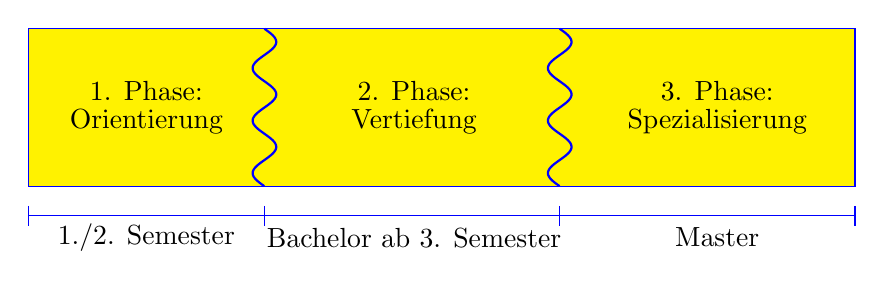
\begin{tikzpicture}
    \path[save path=\boxedpath] (0, 0) -- (0, 2) -- (10.5, 2) -- (10.5, 0) -- (0, 0);
    \filldraw[yellow][use path=\boxedpath];
    \draw[blue][use path=\boxedpath];
    % \path[draw,blue] (3.5, 0) -- (3.5, 2);
    % \path[draw,blue] (7.5, 0) -- (7.5, 2);
    \draw[domain=0:2, smooth, samples=100, thick, blue] plot ({0.15 * sin(3 * pi * \x r) + 3}, {2 - \x});
    \draw[domain=0:2, smooth, samples=100, thick, blue] plot ({0.15 * sin(3 * pi * \x r) + 6.75}, {2 - \x});
    \path[draw,blue] (0, -0.375) -- (10.5, -0.375);
    \draw[blue] foreach \x in {0, 3, 6.75, 10.5} { (\x, -0.25) -- (\x, -0.5) };
    \node at (1.5, 1) {\shortstack{1. Phase:\\Orientierung}};
    \node at (4.9, 1) {\shortstack{2. Phase:\\Vertiefung}};
    \node at (8.75, 1) {\shortstack{3. Phase:\\Spezialisierung}};
    \node at (1.5, -0.65) {1./2. Semester};
    \node at (4.9, -0.65) {Bachelor ab 3. Semester};
    \node at (8.75, -0.65) {Master};
  \end{tikzpicture}
\end{figure}

\section{Angebotsvielfalt und Spezializierungsoptionen}

Die Anforderung an die Gestaltung des Angebots eines Studiengangs schließt grundsätzlich zwei Forderungen ein:
\begin{enumerate}
  \item Hinreichende fachliche Breite anzubieten, um eine gute Basis zu schaffen.
  \item Die Möglichkeiten, eine gewisse fachliche Tiefe zu erreichen -- sowohl vor als auch speziell in der Vertiefungsphase des Studiums.
\end{enumerate}
Im Folgenden werden die Minimalstandards der Angebotsvielfalt und Spezialisierungsoptionen formuliert:
\begin{enumerate}
  \item Eine Hochschule bietet mindestens Veranstaltungen in Algebra, Analysis und einer weiteren Fachrichtung an.
  \item Wenn eine (weiterführende) Veranstaltung Wissen voraussetzt, welches über den Wissensstand der Studienanfänger*innen hinausgeht, wird zeitnah eine Veranstaltung angeboten, die dieses Wissen zuvor vermittelt.
  \item In mindestens zwei der angebotenen Richtungen gibt es genügend weiterführende Veranstaltungen, so dass eine kontinuierliche Weiterentwicklung der Fähigkeiten und Kenntnisse der Studierenden stattfindet.

  Hierzu gehört: Die Studierenden lernen in mindestens zwei Richtungen ihrer Wahl Zusammenhänge ihres Faches zu überblicken und selbstständig mathematische Methoden auszuwählen und sachgerecht anzuwenden. Desweiteren lernen sie, sich selbstständig in verwandte neue Themen einzulesen und diese nachzuvollziehen.
\end{enumerate}
Diese Forderungen gehen auch von einer gewissen Mobilität, Autonomie und einem Engagement der Studierenden aus; dieses wird von der Hochschule sowohl ermöglicht als auch gefördert.

Es ist nicht Aufgabe der Minimalstandards, einen Fächerkatalog bzw. curriculare Vorschläge darzubieten. Dies geschieht stattdessen im Rahmen der Hochschulen und ihrer Koordination untereinander.

\section{Orientierungsphase}

Die Studierenden kommen an die Hochschule und durchlaufen zunächst eine Orientierungsphase. Während dieser gewöhnen sie sich an das Lern- und Arbeitsniveau der Hochschule und finden sich dort fachlich ein.

In der ersten Phase des Studiums werden die Studierenden an das Fachgebiet herangeführt. Durch Schaffen einer soliden Basis wird sowohl die Vertiefung ausgewählter Themen ermöglicht als auch die Autonomie gestärkt, indem der späteren Auswahl der Spezialthemen ein solides Fundament unterstellt wird.

Hierbei wird auch auf Schwankungen bei den Vorkenntnissen der Studierenden eingegangen, d.h. nach Abschluss der ersten Studienphase sind eventuell vorhandene Mängel erkannt und ausgeglichen.

In der ersten Phase des Studiums wird noch keine Vertiefung erwartet. Hier werden die Richtungen aufgezeigt, erste Schritte innerhalb dieser gegangen und insbesondere an das mathematische Denken und Arbeiten herangeführt. Die Studierenden werden hierbei mit den an der Hochschule behandelten Themengebieten vertraut gemacht (siehe Vorlesungen, Seite 12). \todo{Referenz aktualisieren}

Die Inhalte der Grundlagenmodule Analysis und Lineare Algebra sind an allen Hochschulen vergleichbar um einen Hochschulwechsel zu erleichtern.

\section{Vertiefungsphase}

Die Studierenden haben inzwischen ein fachliches Basisniveau erreicht und können erkennen, welche Vertiefungsmöglichkeiten an der eigenen Hochschule angeboten werden und wie auf diese hingeführt wird. Im Rahmen dieser Studienphase werden sie zur Auswahl der Schwerpunkte befähigt.

In der zweiten Studienphase finden in ausgewählten Richtungen Vertiefungen statt; eine weitere Spezialisierung der Studierenden wird vorbereitet. Um den Studierenden Vertiefungen in verschiedene Richtungen zu ermöglichen, unterstützt die Hochschule in dieser Phase auch Standortwechsel. Bei diesen werden bereits erbrachte gleichwertige Leistungen im Sinne der Landeshochschulgesetze anerkannt. Bei abweichenden Studiengängen müssen aber auch die Studierenden Aufwand einplanen um sich dem Curriculum der neuen Hochschule anzupassen.

Ein Studienwechsel wird durch die Hochschule zumindest soweit unterstützt, dass die Fachberatung auf Anfrage Studierender Informationen über die gewünschte Vertiefung an anderen Hochschulen bereitstellt. Die Hochschule, an die gewechselt wird, stellt auf Anfrage klar, welche Leistungen anerkannt werden und welche Leistungen nachzuholen sind.

In dieser Phase werden fachliche Breite und Tiefe gefördert sowie ein Studienabschluss erlangt.

\section{Spezialisierungsphase}

Studierende der dritten Phase sind in der Lage, selbstständig wissenschaftlich zu arbeiten sowie autonom eine Spezialisierung auszuwählen und das eigene Lernen voranzutreiben. Nach der dritten Phase besitzen sie die Fähigkeit, mathematische Methoden und wissenschaftliche Erkenntnisse selbstständig anzuwenden.

Hierbei wird den Studierenden ermöglicht, sich in den gewählten Richtungen weiter zu vertiefen.

Ist keine dritte Phase vorhanden, kann mit Abschluss der zweiten Phase ohne Verlängerung der Gesamtstudienzeit die dritte Phase an einer anderen Hochschule
absolviert werden. Informationen über geeignete Hochschulen werden den Studierenden rechtzeitig bekannt gegeben.

\section{Kontinuität}

Ein Studium ist, wie in den Landeshochschulgesetzen vorgesehen, in Regelstudienzeit absolvierbar, gleich welche der angebotenen Richtungen gewählt werden.

Aufeinander aufbauende Studiengänge sind in Regelstudienzeit absolvierbar; insbesondere wirkt sich der Übergang von einem Studiengang in einen darauf aufbauenden nicht zwingend verlängernd auf die Gesamtstudienzeit aus.

Die Umsetzung der Studienordnung, insbesondere das Vorlesungsangebot und die Prüfungsordnungen, ist so flexibel gestaltet, dass Abweichungen vom planmäßigen Studienverlauf das Gesamtstudium nicht unverhältnismäßig verlängern. Speziell zieht ein Ausfall von einem Semester höchstens eine Studienzeitverlängerung von zwei Semestern nach sich.

\section{Teilzeitstudium / Studieren mit Kind}

Es wird ein Teilzeitstudium angeboten. Ein Wechsel zwischen Voll- und Teilzeitstudium wird ermöglicht und von der Hochschule unterstützt. Ein Beispielstudienverlauf ist angegeben, bei dem die maximale Arbeitsbelastung pro Semester ein gewisses Höchstmaß (Richtlinie: Alleinerziehender Elternteil) nicht übersteigt. Dabei sind keine besonderen Vorkenntnisse gefordert, insbesondere werden zeitliche und finanzielle Limitationen berücksichtigt.

\section{Prüfungen}

Bei benoteten Modulen wird zu Beginn der einzelnen Veranstaltung(en) die Bewertungsmethode transparent gemacht. Insbesondere gilt für Module, die mehrere Veranstaltungen oder Submodule beinhalten, dass das Prüfungskonzept mit Beginn der ersten Veranstaltung vorgestellt wird. Mit Einverständnis aller Teilnehmenden kann das System auch während des Moduls geändert werden.

Wenn das Nichtbestehen einer Prüfung einen Studienausschluss zur Folge hat, so wird den Studierenden die Möglichkeit gegeben, die Prüfung mindestens zweimal zu wiederholen. Es ist möglich, die Prüfung zügig zu wiederholen oder vorher prüfungsrelevante Veranstaltungen erneut zu besuchen.

Die Prüfungsmodalitäten (u.a. Datum und Dauer) werden mindestens einen Monat vor der Prüfung bekannt gegeben. Dabei ist auf eine angemessene zeitliche Verteilung insbesondere der Pflichtprüfungen zu achten.

Die Abmeldung von einer Prüfung ist mit verhältnismäßigem zeitlichen Vorlauf möglich. Innerhalb eines adäquaten Zeitraums ist der krankheitsbedingte Rücktritt von einer Prüfungsleistung mit angemessenem Aufwand möglich.

Schriftliche Arbeiten werden von Studierenden eigenständig angefertigt, wobei sie von einer fachlich kompetenten Person betreut werden. Die betreuende Person ist zu mindestens einem monatlichen persönlichen Gespräch bereit. Zusätzlich ist sie für kurze Nachfragen erreichbar und stellt sicher, dass diese innerhalb einer Woche beantwortet werden. Das zu behandelnde Thema wird zu Beginn der Arbeit festgelegt. Die geäußerten Interessen werden bei der Vergabe des Themas berücksichtigt. Die Vergabe des Themas erfolgt so rechtzeitig, dass das Studium nicht unnötig verlängert wird. Der Umfang des Themas wird so gewählt, dass die Arbeit im dafür vorgesehenen Zeitrahmen fertiggestellt werden kann.

\section{Kontinuität der Studienordnung}

Allen Studierenden, die in einer Studienordnung beginnen, ist es möglich, in dieser das Studium auch abzuschließen.

Dies gilt insbesondere, wenn die Studienordnung ausläuft. In diesem Fall haben sie für das erfolgreiche Abschließen des Studiums ab dem Zeitpunkt, zu dem keine Neueinschreibung gemäß dieser Studienordnung mehr möglich ist, Regelstudienzeit plus ein Jahr Zeit. Sofern eine neuere Studienordnung existiert, ist es den Studierenden jederzeit möglich, auf diese wechseln. Die bereits erbrachten Leistungen werden gemäß klar formulierten Übergangsregelungen (z.B. einer Äquivalenzliste) anerkannt.

\section{Freiheit des Lernens}

Der Student ist selbstständig und übernimmt Eigenverantwortung. Die Hochschule unterstützt ihn in der Freiheit, seinen Studienverlauf selbst zu gestalten. Das umfasst sowohl die Anordnung der Veranstaltungen als auch die Wahl der Methodik und Sozialform des Lernens, wie z.B. Autodidaktik.

Grundsätzlich widerspricht Anwesenheitspflicht bei Veranstaltungen dem Gedanken der Freiheit des Lernens, einzige Ausnahme können Seminare darstellen. Wenn Zulassungsvoraussetzungen zur Prüfung einer Veranstaltung existieren, dann ist der Umfang angemessen und beschränkt sich auf dieselbe Veranstaltung.

Die Wahl des Zeitpunkts des Studienabschlusses ist den Studierenden überlassen.

\section{Orientierung an den Interessen der Studierenden}

Den Studierenden wird die Möglichkeit gegeben, das Veranstaltungsangebot mitzugestalten. Dies bedeutet, dass in allen Gremien, welche Studien- und Prüfungsordnungen oder die Vorlesungsverzeichnisse beschließen, Studierende mit Stimmrecht vertreten sind. Diese sind durch die Fachschaft zu wählen.
